% !TEX root = ../main.tex

\subsection{Project I - Sensor Tracker}
\label{sec:impl:project:i}

\newcommand{\sti}{\textbf{ST1}}
\newcommand{\stii}{\textbf{ST2}}
\newcommand{\stiii}{\textbf{ST3}}
\newcommand{\stiv}{\textbf{ST4}}

The {\gecko} is well suited for applications that focus on low energy consumption.
Examples of such applications are wearable devices, like the \texttt{fitbit}\footnote{\url{https://www.fitbit.com/}} activity tracker.

The following sections describes an interrupt driven sensor application that was developed for the {\STK}, we refer to this application as the {\tracker}.
The project has an emphasis on low energy consumption and it uses sleep modes to save energy during execution.

\subsubsection{Goal}

The {\tracker} application was developed to compare the {\rust} and {\C} languages against each other, with an emphasis on energy consumption on a bare-metal system.
An energy efficient application is largely concerned with performing its task quick and going to sleep.
Different parts of the {\gecko} gets switched off, depending on the sleep mode the chip is in, and the key to low power consumption is to do as much of the data processing at the lower sleep modes.

% The project specification was developed in order to measure the energy efficiency of the {\rust} language used in an embedded system compared to {\C}.
% Given the design of the Gecko, certain operations like memory transfers can also offload the CPU by using DMA.

\subsubsection{Requirements}

The requirements for the {\tracker} application are summarized in \autoref{tab:project:i:requirements}.
We wanted the application to demonstrate the usage of a wide range of sensors; the required peripherals are available on the two given boards in {\sti}.
The sensors from {\stii} were chosen to be the internal temperature sensor on the {\gecko}, and the humidity sensor and the external temperature sensor that are available on the {\BIO}.
{\stiii} and {\stiv} was chosen because they demonstrate two different use-cases for the {\tracker}.
The first mode demonstrates a self-contained system that collects data, and the second mode shows that the application can be used to provide data to external devices.

\begin{table}[H]
  \centering
  \begin{tabular}{c|p{8cm}}
    \textbf{Requirement} & \textbf{Description} \\
    \hline
     \sti   &
     The application should be made for the {\STK} and utilize the {\BIO} for additional sensors. \\
     \stii  &
     The application should collect \emph{samples} of temperature and humidity from various peripherals at timed intervals. \\
     \stiii &
     The samples should be collected and stored internally in the {\gecko}'s \gls{ram}. \\
     \stiv  &
     The sample data should be made available to an external application with the \gls{usart}. \\
    \hline
  \end{tabular}

  \caption{Requirements for the {\tracker}}
  \label{tab:project:i:requirements}
\end{table}


% \subsubsection{Specification}

% The application should record samples from selected peripherals on the STK and BIO-EXP boards described in \autoref{tab:hw:boards}.
% These samples should be stored internally on the {\gecko}.
% When a computer is connected to the \gls{usart} peripheral on the {\gecko}, the samples should be available over a textual serial interface.

\subsubsection{Implementation}

The application has two modes of operation, sample collection and sample transfer.
The buttons on the {\STK} are used to switch between the two operation modes of the {\tracker}, these modes are shown in \autoref{tab:project:i:buttons}, and described in the paragraphs below.

\begin{table}[H]
  \centering
  \begin{tabular}{l|l|l}
    \textbf{Current Mode} & \textbf{Button Pressed} & \textbf{Action} \\
    \hline
    Collect & PB0 & Go to Transfer \\
    Collect & PB1 & Stay in Collect \\
    Transfer & PB0 & Stay in Transfer \\
    Transfer & PB1 & Go to Collect after current transfer \\
    \hline
  \end{tabular}
  \caption{Operation modes for the {\tracker}}
  \label{tab:project:i:buttons}
\end{table}

\paragraph{Sample Collection}
\label{sec:project:i:sample-collection}

\begin{figure}[H]
  \begin{center}
    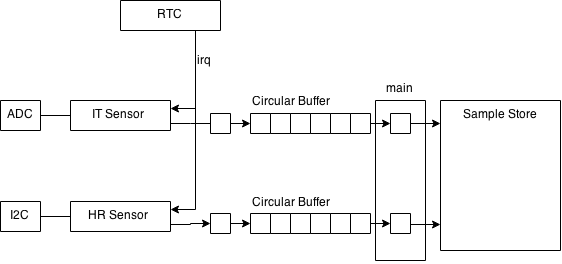
\includegraphics[scale=0.5]{figures/project-i.png}
  \end{center}
  \caption{Sample collection phase}
  \label{fig:project:i:samples}
\end{figure}

The main part of the application, which consists of gathering the samples, was implemented as described in \autoref{fig:project:i:samples}.
The \gls{rtc} clock is set up to generate interrupts each \emph{n} milliseconds.
On each interrupt, a new sample is created by the sensors and pushed into a circular buffer structure.
The main loop, which is executed once after each interrupt has been handled, extracts all the sample currently in the circular buffer and stores them in \gls{ram}.

The sensors\footnote{Sensor \#1 and \#2 are the same sensor, but they are exposed as two different ones by the application.} used in the application are shown in \autoref{tab:project:i:sensors}.
We can see from this table that two additional peripherals need to be configured for the {\tracker}, for the sensors to work properly.
The \gls{adc} is used to convert the internal temperature to a digital value, while the external sensors available on the {\BIO} is retrieved via the {\gecko}'s \gls{i2c} interface.

\begin{table}[H]
  \centering
  \begin{tabular}{ l | l | l | l }
    \textbf{\#} & \textbf{Name} & \textbf{Connection} & \textbf{Measured Data} \\
    \hline
    0 & Internal Temperature & ADC0 & CPU Temperature \\
    1 & Humidity Relative & I2C1 & Room Humidity \\
    2 & Temperature & I2C1 & Room Temperature \\
    \hline
  \end{tabular}
  \caption{Sensors used by the {\tracker}}
  \label{tab:project:i:sensors}
\end{table}

% \paragraph{Sample Transfer}

% The sample transfer mode is implemented by a \gls{cli} over the \gls{usart} serial communication protocol.
% The \gls{cli} offers a read command which is used to read all the samples collected from one of the three sensors described in \autoref{tab:project:i:sensors}

\paragraph{Connecting to the STK}

We use a PC to interface with the {\gecko} over \gls{usart} when the application is in Transfer mode, and the application can then be controlled via a \gls{cli}.
We have used a USB cable with an FTDI chip\footnote{Future Technology Devices International provides chips for serial to USB conversion} to connect with a \gls{usart} on the {\STK}.
\autoref{fig:project:i:connect} shows how the RX (green), the TX (white), and Ground (black) wires are connected.
The application can then be interacted with, with a terminal application like \prog{picocom}\footnote{\prog{picocom} is a serial terminal commonly found in many Unix-like systems}.
Connecting to the device with baudrate 9600 and error correction set to 8-1 (the defaults of \prog{picocom}) will provide access to the {\tracker} \gls{cli}.


\begin{figure}[H]
  \begin{center}
    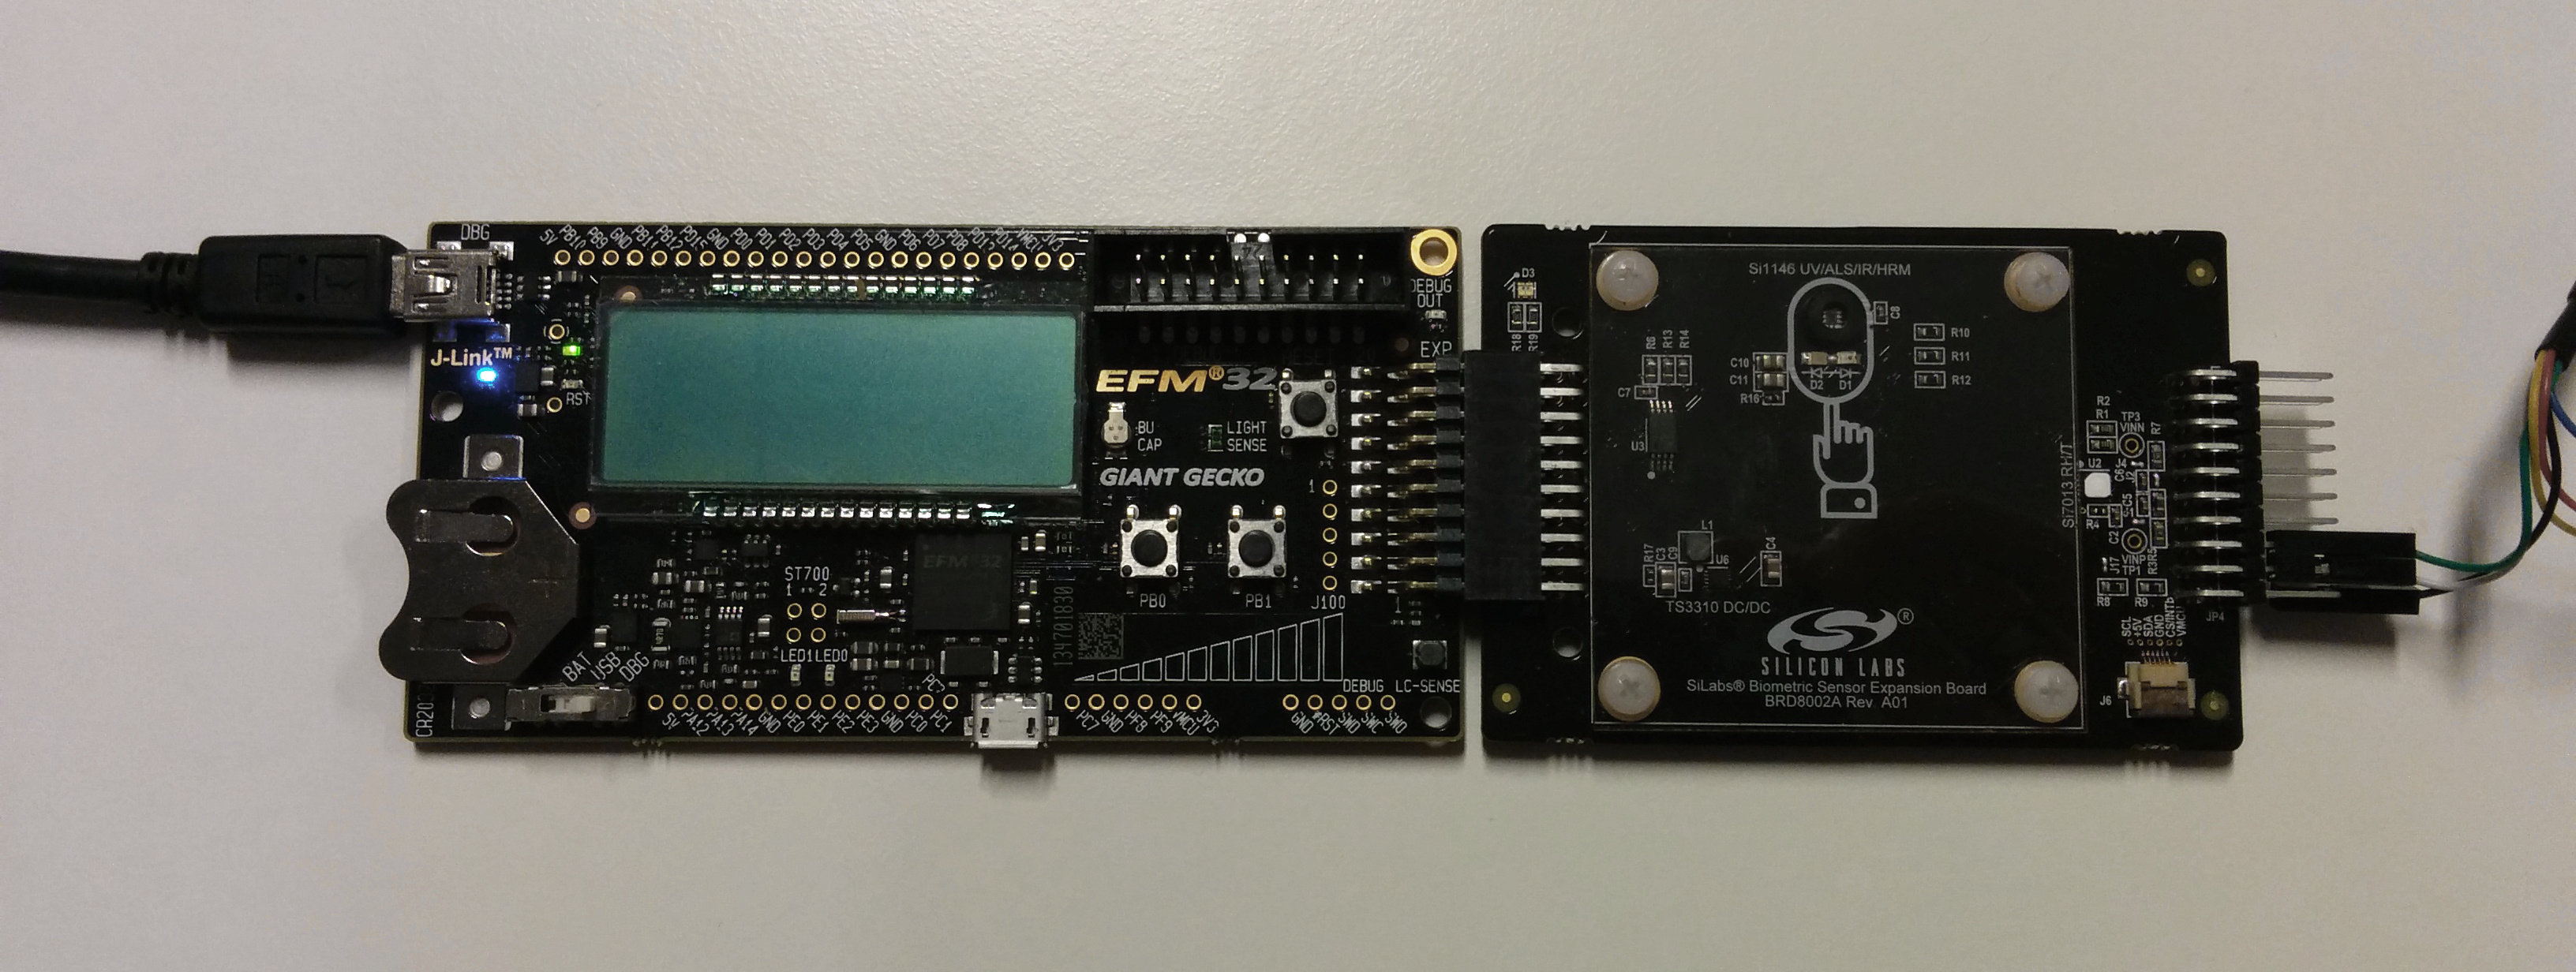
\includegraphics[width=\textwidth]{figures/project-i-connect.jpg}
  \end{center}
  \caption{Connecting to the {\STK}}
  \label{fig:project:i:connect}
\end{figure}


\paragraph{Command Line Interface}

The \gls{cli} of the application contains only a single command; read.
The read command takes one argument, and it is on the format \cmd{r n}, where \emph{n} is the integer 0, 1 or 2.
The command is terminated with a carriage return (i.e. the ASCII symbol \texttt{{\symbol{92}}r}).
All non-conforming commands are ignored by the application.
The \emph{n} parameter is used to select one of the sensors that was presented in \autoref{tab:project:i:sensors}.
Every time a conforming command is sent to the application, it will respond over \gls{usart} with all the data that have been collected by the selected sensor.
A screenshot over how program interaction with the {\tracker} looks like is shown in \autoref{fig:project:i:sample-run}.

\begin{figure}[H]
  \begin{center}
    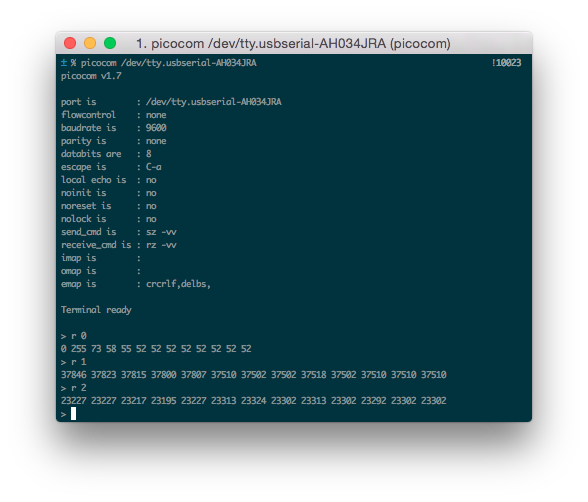
\includegraphics[width=0.62\textwidth]{figures/sensortracker-cli}
  \end{center}
  \caption{Example run of Command Line Interface}
  \label{fig:project:i:sample-run}
\end{figure}
